\documentclass[dwyatte_dissertation.tex]{subfiles} 
\begin{document}

\sloppy

\chapter{The LeabraTI framework: Spatiotemporal prediction with thalamocortical rhythms}
\label{chap:leabrati}

% Plus phase
% + Thalamic burst
% + Cortical amplification of Thalamocortical signals, causes ignition of microcolumn
%   through 2/3->5 and 5b burst to 6
% 	+ Find refs on this -- gating by synchrony. but synchrony is due to inhibition? 
%   + Possibly sensory + intrinsic bursting combo causes gating
%
% Minus phase
% + Next 100-len(bursting) ms characterized by endogenously (L6) driven inputs
% + Thalamus doesn't burst, information already gated down in column, so it becomes primary driver
%   + Should sensory still be let in through feedforward path? Or does it *never* get past L4?
%
% BeierleinFallRinzelEtAl02 - burst > 40 Hz 
% WangSpencerFellousEtAl10 - sync
% FeldmeyerLubkeSilverEtAl02 - sync
% TiesingaFellousSejnowski08 - sync
%
% " Thalamocortical synapses are more effective than intracortical synapses, but they form only a small fraction of the synapses onto L4 stellates."

% TODO
% * microcircuit latencies
% * Nesting of gamma within alpha, and actually is the ``duty cycle'' -- need to reread Spaak, Jensen papers
% * Add shared thalamus to figure and generally fix
% * Begin writing about alpha synchronization and desycnrhonization and how they are related to sensation and prediction -- cite relevant EEG evidence -- but save 		the bulk of this for the EEG section
% * analogies about carrier signals/duty cycles?

\section{Introduction}
%\subsection{Overview of LeabraTI Model}
%
%\begin{figure}
%  \centering\includegraphics[width=6in]{figs/fig_leabra_ti_func}
%  \caption{\footnotesize The temporal evolution of information flow in a LeabraTI model predicting visual sequences, over a period of three alpha cycles of 100 msec each.  The  Deep context maintains the prior 100 msec information while the Superficial generates a prediction (in the minus phase) about what will happen next.  Learning occurs in comparing this prediction with the plus phase outcome, which generates an updated activity pattern in the Super layers.  Thus, prediction error is a temporally extended quantity, not coded explicitly in individual neurons.}
%  \label{fig.leabra_ti}
%\end{figure}

%\begin{figure}
%  \centering\includegraphics[width=4in]{figs/fig_leabra_ti_v1_v2_detailed}
%  \caption{\small Anatomical connectivity supporting the LeabraTI model. Super (II/II) layers have extensive connectivity within and between areas, and do the primary information processing.  Deep layer V integrates contextual information within and between areas, and 5b bursting neurons only update this context signal every 100 msec, driving a new state of firing on the layer VI tonic firing neurons.  These layer VI neurons sustain the context through recurrent projections through the thalamic relay cells (TRC), which also communicate the context up to the Super neurons (via IV) to support generation of the next prediction.}
%  \label{fig.leabra_ti_bio}
%\end{figure}
%
%The LeabraTI model of temporal integration in the neocortex leverages the unique properties of the thalamocortical microcircuit (Figures~\ref{fig.leabra_ti}, \ref{fig.leabra_ti_bio}).  This model makes detailed contact with a wide range of biological and functional data, often with counterintuitive predictions. % and we are not aware of any existing data that clearly contradicts it. 
%Specifically, the two major claims are:
%
%{\bf 1. Time is discretized into roughly 100 msec intervals}, which correspond to the widely observed alpha rhythm in posterior neocortex.  Computationally, this discretization is important for giving the system sufficient time for bidirectional constraint-satisfaction processing to generate reasonable expectations about what will happen next. Because this processing itself takes time, it is not possible to be continuously generating these predictions, and hence the input must be discretely sampled.  Biologically, the properties of the layer 5b deep neocortical neurons, together with dynamics of thalamic neurons, are thought to underlie the generation of the alpha rhythm \abbrevcite{LorinczKekesiJuhaszEtAl09,FranceschettiGuatteoPanzicaEtAl95,BuffaloFriesLandmanEtAl11,LuczakBarthoHarris13}.  Psychologically, there is increasing evidence for a discretization of perception at the alpha scale \abbrevcite{VanRullenKoch03b}. % We review this literature in more detail below.
%
%{\bf 2. Temporal context is sustained in the deep neocortical layers}, while the superficial layers continuously integrate new information, along with this sustained deep context.  % Dean: this might not be the right place to describe the computation in detail
%Specifically, we argue that the burst-firing dynamics of the layer 5b neurons result in two phases of activity in the deep layers, corresponding to the minus and plus phases of the Leabra algorithm.  The 5b neurons burst fire in the plus phase, driving the updating of downstream layer 6 neurons, which then drive input back down to the thalamus, which then comes back up to the same cortical area, both to layer 6 and up to layer 4 and from there onto the superficial layers (Figure~\ref{fig.leabra_ti_bio}). However, in the minus phase, the 5b neurons are relatively quiescent, and this protects the layer 6 neurons from further influences, enabling them to continue to represent the temporal context from the prior plus phase.  The sustained firing of this layer 6 signal then feeds into the superficial layers, which integrate this prior temporal context with information from all over the rest of the cortex (via inter-areal bidirectional excitatory projections), to produce an expectation about what will happen next.  Then, whatever does happen, happens, and that constitutes the plus phase against which the prior expectation is compared, to drive error-driven learning.  The STDP-based {\em XCAL} learning mechanism in Leabra \cite{OReillyMunakataFrankEtAl12} automatically computes this comparison in a biologically-plausible fashion.  This minus-plus phase oscillation at the alpha frequency thus constitutes the fundamental ``clock cycle'' of cortical computation, according to this framework.



% TODO: Overview of the model with major predictions instead, pull from above text from full TI paper

This chapter describes the LeabraTI (Temporal Integration) framework, which is a mechanistic description and general model of how prediction and temporal integration works in the brain. It is closely related to the Simple Recurrent Network (SRN) \cite{Elman90,Servan-SchreiberCleeremansMcClelland91}  a neural network architecture that explicitly represents temporally lagged information in discrete ``context'' units whose activity gets integrated with more current information to predict what happens in the next time step (Figure \ref{fig:srn_circuit}a). This method of copying a contextual representation from an intermediate representation at discrete intervals was originally shown to be a robust way to leverage error-driven learning to represent latent temporal structure in auditory streams and artificial grammars. More generally, the SRN's explicit representation of temporally lagged context can capture the latent structure of any stimulus that varies systematically over time, making it a good basis for a generic prediction and temporal integration mechanism.

LeabraTI differs in several key ways from the classical SRN architecture, primarily in the way context is represented and used in predictive processing. These differences are due to biological constraints imposed by the microcircuitry of the neocortex, and thus form a number of testable predictions that can be used to evaluate the validity of the LeabraTI framework. The central prediction of LeabraTI is that temporally lagged context is represented by deep (Layer 6) neurons, which is possible in part to the bifurcation of intra-areal and inter-areal processing streams. As neural processing is a continuous operation, LeabraTI requires a regular interval over which to integrate deep context and make predictions, which is suggested to be approximately every 100 ms. Predictions are made by driving superficial (Layers 2 and 3) neurons with the state of deep neurons through the intra-areal pathway, which is interlaced with standard peripheral sensory inputs over a total period that is also 100 ms. The strong 100 ms dependency in LeabraTI corresponds to the brain's alpha rhythm, which has been studied extensively using scalp EEG (\nopcite{MathewsonGrattonFabianiEtAl09,BuschDuboisVanrullen09,GouldRushworthNobre11,RohenkohlNobre11}; \abbrevnopcite{MathewsonPrudhommeFabianiEtAl12,BelyusarSnyderFreyEtAl13}; \nopcite{VanRullenDubois11}). 

\textbf{TODO: Foreshadow structure of chapter...}

% srn/microcircuit fig
\begin{figure}[h!]
\begin{center}
\begin{tabular}{ll}
\textbf{A} & \textbf{B} \\
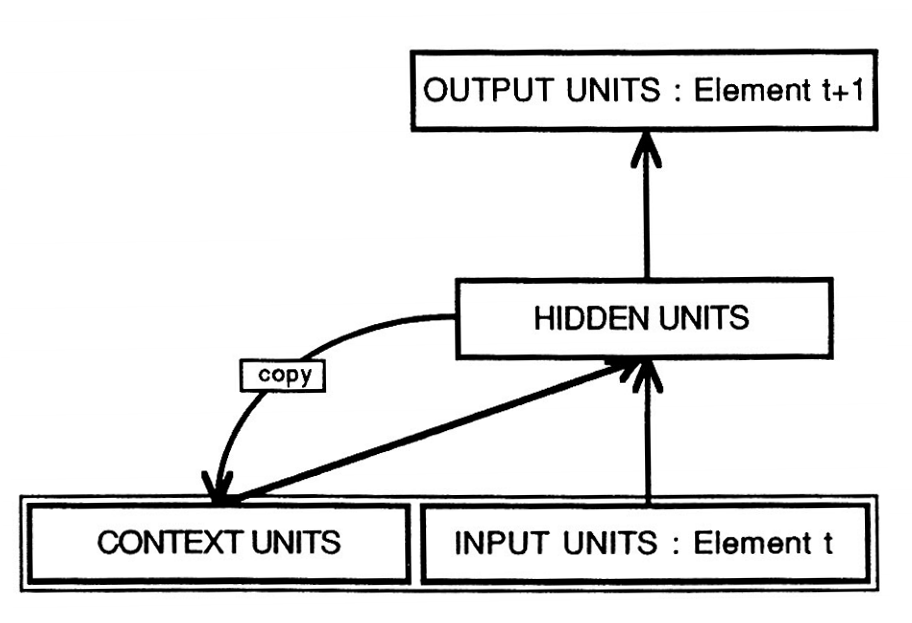
\includegraphics[width=80mm]{figs/chap_leabrati/srn_scm.png} &
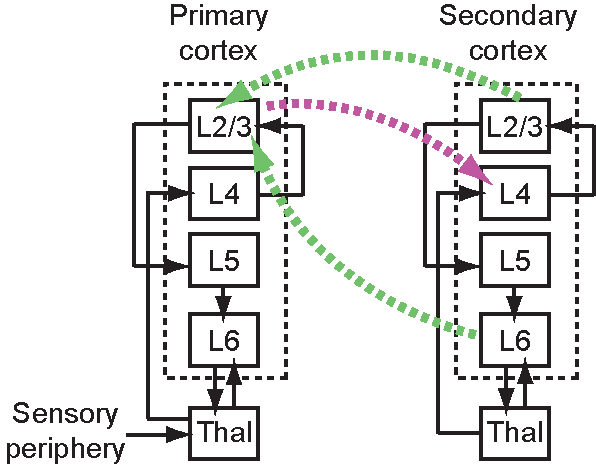
\includegraphics[width=80mm]{figs/chap_leabrati/microcircuit_horiz.pdf} \\
\end{tabular}
\end{center}
\caption{The Simple Recurrent Network (SRN) and microcircuitry of the neocortex}{\textbf{A}: The SRN represents temporal information explicitly using discrete context units that are updated once per time step. Context is integrated with more current inputs to predict information at the subsequent time step. Reproduced from \protect\incite{Servan-SchreiberCleeremansMcClelland91}. \textbf{B}: The neocortex is laminated with canonical circuitry between neurons across layers and between areas. Intra-areal connections are shown in black with inter-areal feedforward connections in purple and feedback connections in green.}
\label{fig:srn_circuit}
\end{figure}

\section{LeabraTI biological details}
\subsection{Laminar structure and microcircuitry of the neocortex}
% instead of writing a damn mystery story, just note commonalities across 2 figures -- thalamus can be driven by either "input" or L6. will need to modify dacosta/martin figure 

A salient feature of the brain, and potential clue in realizing how an SRN-like computation might be carried out in biological neural circuits, is the laminar structure prevalent across the neocortex (Figure \ref{fig:srn_circuit}b). Incoming information from the sensory periphery is transmitted through the thalamus and targets Layer 4 neurons in the primary sensory cortices (e.g., V1). From there, Layer 4 neurons propagate spikes to superficial neurons (Layers 2 and 3) which in turn target Layer 4 neurons of higher-level cortices, forming the prominent corticocortical feedforward pathways that subserve visual and auditory recognition \cite{FellemanVanEssen91}. Corticocortical feedback originates in superficial layers or Layer 6 of the higher-level cortex and generally terminates on superficial neurons of the lower-level cortex \cite{RocklandPandya79}. In addition to these interareal pathways, there exists a canonical microcircuit of the form Layer 4 $\rightarrow$ Layer 2/3 $\rightarrow$ Layer 5 $\rightarrow$ Layer 6 that routes spike propagation through the local neuronal structure \cite{DouglasMartin04,ThomsonLamy07}. This microcircuit forms the core computational unit of LeabraTI, as will be described in this and the following sections.

The importance of the local microcircuit was first suggested by Vernon Mountcastle in his proposal regarding the gross columnar organization of the neocortex \cite[see][for a comprehensive review]{Mountcastle97}. Mountcastle's proposal states that microcolumns composed of around 80-100 neurons extending vertically through all six lamina with canonical circuitry form the core repeating structure of the neocortex. Neurons within a single micrcolumnnar circuit possess nearly identical receptive field tunings across lamina while neurons in neighboring microcolumns (radial separation greater than 600 \SI{}{\micro\meter}) possess very different receptive field tunings but contribute to the higher-order macrocolumn (i.e., hypercolumn) structure \cite{HubelWiesel77,Jones00}. Microcolumns have been identified in a variety of neural systems with this electrophysiological mapping and are also prominently visible under Nissl staining. Despite this evidence for their structural existence, any function of the microcolumn aside from an organizing principle remains debated \cite{BuxhoevedenCasanova02,HortonAdams05}.

LeabraTI provides a computational role for the microcolumn, by mapping an SRN-like computation onto their Layer 4 $\rightarrow$ Layer 2/3 $\rightarrow$ Layer 5 $\rightarrow$ Layer 6 circuit. In this mapping, superficial neurons continuously integrate feedforward and feedback interareal synapses to process current information. Layer 2/3 $\rightarrow$ Layer 5 $\rightarrow$ Layer 6 provides an intraareal pathway for explicitly representing temporal context deep layers, which are relatively isolated from nonlocal inputs. There is also appropriate circuitry for recirculating this context through the local microcolumn via Layer 4 to drive the learning of temporal associations. This basic idea provides a concise explanation for the strong degree of isotuning throughout a single microcolumn, as deep neurons need to represent the same information as superficial neurons except at a delayed interval.

More generally, LeabraTI's dichotomy of continuous integration in superficial layers and periodic updating of deep layers receives strong support by the literature. Recent studies that have employed depth electrodes to simultaneously record from multiple layers within a patch of cortex have indicated that superficial layers exhibit spectral power at much higher frequencies than deep layers. \incite{BuffaloFriesLandmanEtAl11} recorded responses from ventral visual sites V1, V2, and V4 in awake, behaving monkeys during a simple directed attention task, finding a dissociation in spike coherence frequency in superficial (gamma spectrum, peak $\sim$50 Hz) and deep layers (alpha spectrum, peak $\sim$10 Hz). A similar experimental paradigm expands on these findings by demonstrating cross-frequency coupling between gamma and alpha spectra localized to superficial and deep layers, respectively \cite{SpaakBonnefondMaierEtAl12}. % say something about modulation here
The cross-frequency coupling is characterized by a clear nesting of gamma activity within alpha cycles, suggesting that deep neurons' alpha activity might subserve a general pacemaker mechanism. In the context of LeabraTI, this pacemaker property is important to ensure the regular updating of context through deep layers and temporally predictable reintegration with more current information.

In summary, the laminocolumnar organization of the neocortex provides the dual pathways necessary for continuous information processing and the SRN's explicit temporal context representation. One question that remains, however, concerns the 10 Hz alpha periodicity of deep neurons. The Layer 4 $\rightarrow$ Layer 2/3 $\rightarrow$ Layer 5 $\rightarrow$ Layer 6 microcircuit only contains four synapses including the thalamus and intracolumnar monosynaptic latencies for regular spiking neurons are on the order of 5 ms or faster \cite{Armstrong-JamesFoxDas-Gupta92,LumerEdelmanTononi97}. This relatively small amount of tissue, if driven with constant input, would cause deep neurons to spike at a rate much faster than 10 Hz. How such a circuit could produce the strong alpha power observed in recent depth recordings is described next. % NO MYSTERY STORY DAMMIT

% also need to raise problem of how error-driven learning works -- requires pacemaker (motivate next section)

\subsection{Pacemaker properties of Layer 5 and thalamic bursting neurons} % need a better title
% combine everything below into one section

% L5/L6
%
% 5a regular spiking and 5b intrinsic bursting distinction
% Layer 6 relatively isolated from extra columnar inputs
% 5b -> 6 integration, 6 is Regular spiking output through, maintained by thal

% thalamus has similar intrinsic bursting properties. need to re-read Lorincz paper, but can talk about relay mode and such
% don't talk about alpha rhythm just yet
% but do talk about other evidence regarding prediction/sensation e.g., phase locking with environmental stim

Layer 5 neurons can be roughly divided into 5a and 5b subtypes \cite{ThomsonLamy07}. Layer 5a neurons have relatively small cell bodies and exhibit ``regular spiking'' depolarization responses. They collect input from other Layer 5a neurons and pass it to 5b neurons and thus, likely play a simple information integration role. Layer 5b neurons, in contrast, have larger cell bodies and exhibit ``intrinsic bursting'' properties at $\sim$10 Hz when over threshold (\nopcite{ConnorsGutnickPrince82,SilvaAmitaiConnors91}; \abbrevnopcite{FranceschettiGuatteoPanzicaEtAl95}). % FlintConnors96 -- relation of NMDA to L5 alpha bursts

Thalamic neurons...


Layer 5b neurons project to Layer 6 whose neurons can also be roughly divided into corticocortical (CC) and corticothalamic (CT) subtypes \cite{Thomson10}.

Both Layer Layer 6 CC neurons have properties similar to Layer 5a neurons -- they collect inputs from other Layer 6a neurons and pass it to Layer 6 CT neurons. Layer 6 CT neurons project specifically to the thalamus and also receive direct thalamic input forming a small circuit. They have 

This rhythmic firing has been shown to persist even with constant sensory stimulation \textit{in vivo} \cite{LuczakBarthoHarris13}, suggesting that Layer 5 neurons' alpha rhythmicity could implement a roughly 10 Hz gating function for spikes relayed to Layer 6 neurons. % get rid of gating, change to updates/periodicities
% need to talk about two types of layer 6 neurons and how one of them integrates broader context of L5 bursts -- make sure this is compatible with biology i.e., multiple L5b guys project to 1 of the broad RF L6 guys

Thus, Layer 6 specifically becomes the neural substrate of the SRN's temporally lagged context representation, representing information that is, on average, one alpha cycle (approximately 100 ms) in the past. This contextual storage occurs at an automatic interval due to the intrinsic pacemaking properties of Layer 5 neurons, and might implement a reference frame that essentially would allow the brain to know \textit{when} to anticipate inputs. As such, intrinsic oscillations have been shown to phase lock to environmental stimulation \cite{WillBerg07,LakatosKarmosMehtaEtAl08,SchroederLakatos09,StefanicsHangyaHernadiEtAl10}, ensuring environmental events coincide with key events like Layer 5 bursts in cortex. % need to unpack this entrainment idea and motivate prediction without corruption

%\subsection{Thalamic gating and prediction in superficial layers}
% Spaak: within the lower frequency alpha oscillations and an inverse relationship in which alpha attenuation resulted in higher amplitude and longer lasting gamma activity (and vice versa)

Layer 6 sends axons toward the thalamus, completing the microcircuit within the local column and allowing the temporally lagged Layer 6 information to integrate with more current Layer 4 inputs. There also exists a direct connection between Layer 6 and Layer 4, that could be used for this purpose, although it has been noted as being weak compared to other intracolumnar connections \cite{HirschMartinez06b}. In either case, temporal associations could be created by simple Hebbian learning mechanisms that track high probability co-occurences across past and present events. % can draw analogies here to more biological trace rule

The Leabra algorithm \cite{OReillyMunakata00,OReillyMunakataFrankEtAl12}, however, also makes use of powerful error-driven learning (in addition to more standard Hebbian learning). In the context of temporal integration, error-driven learning would allow computation of error signals based on the difference between what is predicted to happen at a given moment (given the previous moments context as an input) and what actually happens. However, this computation requires that both the prediction and the actual sensation are represented subsequently within a single alpha cycle, which is not possible if the sensory periphery is always transmitting incoming inputs. To resolve this issue, the LeabraTI framework posits a mechanism to modulate or even block the transmission of inputs from the sensory periphery. A subset of cells in the thalamus exhibit alpha spectrum bursting properties similar to that of Layer 5 neurons (\nopcite{LopesdaSilva91}; \abbrevnopcite{HughesLorinczCopeEtAl04}; \nopcite{LorinczCrunelliHughes08}; \nopcite{LorinczKekesiJuhaszEtAl09}), and thus perhaps perform a similar gating function. Specifically, these neurons appear to shift the balance of inputs to Layer 4 and superficial neurons between exogenous environmental inputs and endogenous inputs local to the microcolumn. % No direct evidence of this (i.e., they don't ``appear to'')

When environmental inputs are downmodulated or blocked, Layer 6 context relayed via the thalamus is the dominant input to the microcolumn, which can be used to predict the incoming sensory event during the latter part of the alpha cycle. Importantly, during both the prediction and sensation phases, feedforward and feedback projections are constantly transmitting between lower and higher cortical areas. As previously mentioned, these projections originate and terminate predominantly in superficial layers, boosting their spike coherence to higher frequency spectra. This could potentially explain the differentially high gamma power in superficial layers compared to deep layers, and provides a compelling link between gamma oscillations and predicting specific details about the next sensory event.

\subsection{Summary of LeabraTI computation}
The overall computation of LeabraTI is shown in Figure \ref{fig:leabrati_comp} and summarized here. When thalamic cells burst (roughly every 100 ms), information from the sensory periphery is the primary driving force for Layer 4 neurons in primary cortex. This information is relayed downstream to higher-level cortical areas via the strong feedforward Layer 4 $\rightarrow$ Layer 2/3 $\rightarrow$ Layer 4 pathway \cite{FellemanVanEssen91}. Within the local microcolumn, Layer 5 neurons integrate this information, until thalamic bursting quiets (generally around 50 ms). At this point, Layer 5 cells burst, sending outputs to Layer 6 and shifting and inputs to the microcolumn  endogenously. The information represented by Layer 6 neurons is temporally lagged (from the previous 50 ms) and is relayed to Layer 4 via non-bursting (regular spiking) thalamic neurons or via the direct Layer 6 $\rightarrow$ Layer 4 connection (not pictured in Figure \ref{fig:leabrati_comp}), and might be maintained by reciprocal thalamocortical drive back to Layer 6. This information can be used as a prediction as to what will happen next when thalamic bursting resumes and veridical sensory information serves as the input once again. In the context of Leabra's error-driven learning these two phases correspond to the plus phase (sensation) and minus phase (prediction), which can be used to compute a sensory prediction error signal. This error signal modifies Layer 5 $\rightarrow$ Layer 6 synapses to minimize differences between predictions and sensations over time.

Critically, for the LeabraTI computation to work, thalamic and Layer 5 oscillatory phases need to have an approximately antiphase relationship in order for the error-driven learning scheme described here to work so that Layer 2/3 neurons can represent the current moment's prediction with Layer 6 context as their primary input and then subsequently represent the veridical sensory input while Layer 5 neurons are queuing up the next contextual event. Such a relationship has not yet been shown yet, but very few studies have recorded simultaneously from thalamic and cortical neurons in \textit{in vivo} in the awake behaving animal. It is also possible that the brain implements error-driven learning in such a way that does not require representing predictions and sensations temporally interleaved on the same neural substrate or even that the brain accomplishes temporal integration completely without supervision, which in case thalamic gating is not required.

% leabrati computation
\begin{figure}[h!]
\begin{center}
\begin{tabular}{ll}
a) \hspace{76mm} b) \\
\multicolumn{2}{c}{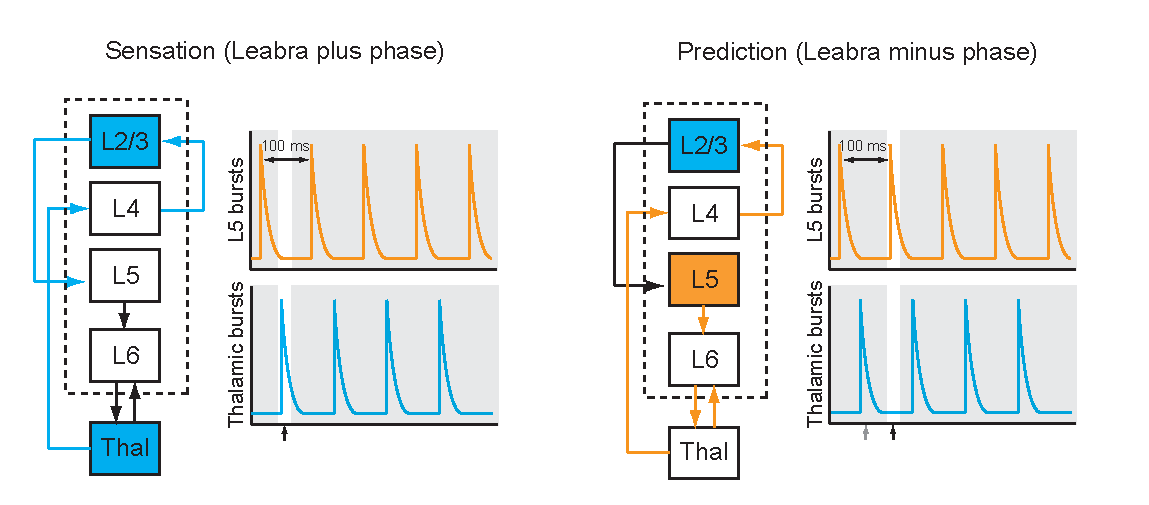
\includegraphics[width=160mm]{figs/chap_leabrati/leabrati_comp.pdf}} \\
\end{tabular}
\end{center}
\caption{The LeabraTI model computation.}
\label{fig:leabrati_comp}
\end{figure}


\section{Relation to other frameworks}
% SRN
% *  need to talk about "copy" operation and inversion of it makes an autoencoder, more consistent with bio?
% Context needs to have a "smart" representation -- this means one of two things: it can be a direct copy of the Hidden layer (as in a standard SRN), effectively borrowing all the learning that shapes the Hidden layer, or it can have its own learned representation, in which case it needs some kind of useful training signal.
% 'NOT a direct copy of the contents of the microcolumn itself but rather the sustained reflection of the net input from the broader context back to the microcolumn. Consistent with this, 6CTC guys have very broad RF's relative to their own microcolumn, and integrate information widely. The combined effects of 5b BI and 6 CC rapid depression result in a very phasic update of the 6CTC cells (on the alpha cycle). The output of the 6CTC's has strong mGluR concentrations, leading to longer-lasting effects, combined with the facilitating synaptic dynamics, resulting in the sustained delivery of this contextual netin to the rest of the microcolumn units via sustained influence on thalamus etc.
% more like a temporal autoencoder

% Predictive coding
% Has been described for single stimuli, but not temporal sequences. Still, compatible with temporal idea, but very different predictions -- need to re-read Bastos paper to determine how prediction error is manifested in super/deep layers and how it would work over time. Still, there is the standard Leabra/predictive coding difference to talk about 
% same ``delta'' signal (predicted - actual) but interleaved over time instead of a residual error  code -- different predictions, esp in terms of activation levels (see predictive remapping)

% To generate reasonable expectations, it is essential to sustain and integrate information from the past
\section{LeabraTI testable predictions}
% short bit about general predictions regarding synchronicity between layers, latencies and how readout should be 100 ms in past, etc.
% but focus of this section will be on EEG predictions
% * Alpha entrainment, classic alpha effects -- see RFI for topics to hit
% * 	Nobre, Busch, VanRullen, Mathewson, etc.
% * 	prediction/sensation interleaving, basic evidence for this, to be tested further with my experiments
% *		Role of attention vs. prediction
\textbf{TODO}


\bibliographystyle{apa}
\bibliography{ccnlab}

\end{document}